% Source: gradient.tex
\begin{notechapter}
\chapter{The Gradient and the Tangent Space}\label{ch:gradient-tangent-space}
\chaptersubtitle{Why the gradient naturally lives in the tangent space}

\section{The Fundamental Question}

A crucial question arises: if the gradient lives in the tangent space, how can it give the direction of steepest ascent \emph{in the surface}? Wouldn't it need to be projected onto the surface?

The beautiful answer is: \textbf{No projection is needed} because the tangent space \textbf{is} the mathematical representation of directions within the surface.

\section{The Tangent Space as ``Within-Surface'' Directions}

\subsection{Definition via Curves}

\begin{definition}[Tangent Space via Curves]
A vector $v$ belongs to $T_p M$ if and only if there exists a smooth curve $\gamma: (-\epsilon, \epsilon) \to M$ with:
\begin{itemize}
\item $\gamma(0) = p$ (curve passes through $p$)
\item $\gamma(t) \in M$ for all $t$ (curve stays on the manifold)  
\item $\gamma'(0) = v$ (vector is the curve's velocity)
\end{itemize}
\end{definition}

This means: \textbf{Every vector in $T_p M$ represents an actual direction you can move while staying on the manifold}.

\subsection{The Riemannian Metric}

To measure lengths and angles within the tangent space, we need:

\begin{definition}[Riemannian Metric]
A \textbf{Riemannian metric} on a manifold $M$ is a smooth assignment of an inner product $g_p$ to each tangent space $T_p M$.
\end{definition}

The metric $g_p$ tells us how to compute:
\begin{itemize}
\item Lengths: $\|v\| = \sqrt{g_p(v,v)}$
\item Angles: $\cos\theta = \frac{g_p(u,v)}{\|u\|\|v\|}$
\item Dot products within the surface
\end{itemize}

\section{The True Definition of the Gradient}

\begin{definition}[Gradient via Riemannian Metric]
The gradient $\nabla f(p)$ is the unique vector in $T_p M$ satisfying:
\[
g_p(\nabla f(p), v) = df_p(v) \quad \text{for all } v \in T_p M
\]
where $df_p: T_p M \to \mathbb{R}$ is the differential of $f$.
\end{definition}

\subsection{Why This Works}

This definition ensures that:

\begin{enumerate}
\item $\nabla f(p) \in T_p M$ by construction
\item The directional derivative in direction $v$ is $D_v f = g_p(\nabla f(p), v)$
\item The steepest ascent direction maximizes $D_v f$ subject to $g_p(v, v) = 1$
\end{enumerate}

\begin{theorem}[Steepest Ascent Property]
Among all unit vectors $v \in T_p M$ (where $g_p(v, v) = 1$), the directional derivative $D_v f$ is maximized when:
\[
v = \frac{\nabla f(p)}{\|\nabla f(p)\|}
\]
where $\|\nabla f(p)\| = \sqrt{g_p(\nabla f(p), \nabla f(p))}$.
\end{theorem}

\begin{proof}
By definition, $D_v f = g_p(\nabla f(p), v)$. By the Cauchy-Schwarz inequality for the inner product $g_p$:
\[
|g_p(\nabla f(p), v)| \leq \|\nabla f(p)\| \cdot \|v\| = \|\nabla f(p)\|
\]
with equality if and only if $v$ is parallel to $\nabla f(p)$; the maximum value $+\|\nabla f(p)\|$ is reached for $v$ pointing in the \emph{same} direction as $\nabla f(p)$ (and the minimum for the opposite direction), assuming $\nabla f(p) \neq 0$.
\end{proof}

\section{Concrete Example: The Sphere}

Let $M = S^2$ (the unit sphere) and $f$ = temperature on the sphere.

\begin{itemize}
\item At point $p$ on the sphere, $T_p S^2$ is the tangent plane
\item Every vector in $T_p S^2$ represents a direction you can actually walk on the sphere
\item The Riemannian metric is the dot product restricted to the tangent plane
\item $\nabla f(p)$ is computed using this restricted dot product
\item Therefore, $\nabla f(p)$ automatically points in a physically realizable walking direction
\end{itemize}

\begin{figure}[h]
\centering
\begin{tikzpicture}[scale=1.5]
% Sphere
\draw[thick] (0,0) circle (1.5cm);
% Point
\filldraw (1.06,1.06) coordinate (P) circle (1pt) node[above right] {$p$};
% Tangent plane
\draw[blue, thick, rotate around={45:(1.06,1.06)}] 
    (1.06,1.06) -- ++(0.8,0) -- ++(0,0.8) -- ++(-0.8,0) -- cycle;
% Gradient vector
\draw[->, thick, red] (P) -- ($(P)+(0.5,-0.5)$) node[right] {$\nabla f(p)$};
% Some possible directions in tangent space
\draw[->, thick, green!60!black] (P) -- ($(P)+(0.3,0.6)$);
\draw[->, thick, green!60!black] (P) -- ($(P)+(-0.4,0.4)$);
% Level curves
\draw[green, thick] (0.8,1.2) to[out=-30,in=150] (1.4,0.8);
\draw[green, thick] (0.6,1.0) to[out=-30,in=150] (1.6,0.6);
\node[blue, right] at (1.3,1.3) {$T_p S^2$};
\end{tikzpicture}
\caption{On a sphere, the gradient $\nabla f(p)$ lies in the tangent plane $T_p S^2$ and points in the direction of steepest ascent along the surface.}
\end{figure}

\section{When Would Projection Be Needed?}

The confusion often comes from thinking about \textbf{embedded manifolds}. Consider:

\begin{itemize}
\item A function $F: \mathbb{R}^3 \to \mathbb{R}$ (temperature in 3D space)
\item Restricted to $M = S^2$ (the sphere)
\end{itemize}

The \textbf{ambient gradient} $\nabla F(p)$ (computed in $\mathbb{R}^3$) might point out of the sphere. In this case, you would project it onto the tangent space to get the \textbf{intrinsic gradient}.

However, when we say $f: M \to \mathbb{R}$ from the beginning, we mean $f$ is defined \textbf{on the manifold}, and its gradient is defined intrinsically using the manifold's geometry.

\section{The Beautiful Summary}

The tangent space formalism is powerful because:

\begin{enumerate}
\item \textbf{$T_p M$ IS the space of ``within-surface'' directions}
\item \textbf{The Riemannian metric $g_p$ encodes the surface geometry}
\item \textbf{The gradient is defined using $g_p$, so it automatically respects the surface geometry}
\item \textbf{Therefore, $\nabla f(p)$ already points in a physically realizable direction within the surface}
\end{enumerate}

The gradient doesn't need projection onto the surface \textbf{because it was born in the tangent space}, which is exactly the mathematical representation of ``directions within the surface.''

This is why differential geometry is so elegant: the abstract definitions automatically give us geometrically correct answers.

\section*{Key Insight}

The gradient $\nabla f(p)$ gives the direction of steepest ascent \emph{in the surface} precisely \textbf{because} it lives in the tangent space $T_p M$, and $T_p M$ \textbf{is} the space of possible directions within the surface.

No projection is needed—the mathematics was designed to automatically handle this!

\section{The Single Variable Case Revisited}

\subsection{The Hidden Identification}

In single-variable calculus, there's a subtle identification that often goes unnoticed:

\begin{itemize}
\item We have a function $f: \mathbb{R} \to \mathbb{R}$
\item At point $a$, the derivative $f'(a)$ lives in $T_a\mathbb{R}$
\item But we casually say "$f'(a)$ tells us which way to move on the x-axis"
\end{itemize}

This works because of the natural isomorphism $T_a\mathbb{R} \cong \mathbb{R}$.

(To be precise, what calculus gives us directly is the \emph{differential} $df_a: T_a\mathbb{R} \to \mathbb{R}$, $v \mapsto f'(a)\,v$, a linear form, i.e.\ an element of the cotangent space $T_a^*\mathbb{R}$. The tangent \emph{vector} $f'(a) \in T_a\mathbb{R}$ is the gradient, obtained from $df_a$ through the metric as in the definition above; with the standard metric of $\mathbb{R}$ both are represented by the same number $f'(a)$. The next chapter develops this distinction.)

\subsection{Visualizing the Correct Picture}

\begin{figure}[h]
\centering
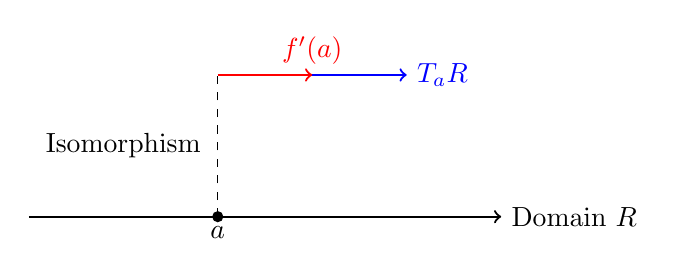
\begin{tikzpicture}[scale=1.2]
% x-axis (domain)
\draw[->, thick] (0,0) -- (5,0) node[right] {Domain $\mathbb{R}$};
\filldraw (2,0) circle (1.5pt) node[below] {$a$};

% Tangent space above the point
\draw[->, thick, blue] (2,1.5) -- (4,1.5) node[right] {$T_a\mathbb{R}$};
\draw[->, thick, red] (2,1.5) -- (3,1.5) node[above] {$f'(a)$};

% Connection
\draw[dashed] (2,0) -- (2,1.5);
\node at (1,0.75) {Isomorphism};
\end{tikzpicture}
\caption{The derivative $f'(a)$ lives in the tangent space $T_a\mathbb{R}$, which is isomorphic to but distinct from the domain $\mathbb{R}$.}
\end{figure}

\subsection{What's Really Happening}

The correct interpretation is:

\begin{enumerate}
\item The derivative $f'(a) \in T_a\mathbb{R}$ is a \textbf{tangent vector} (a velocity)
\item Through the isomorphism $T_a\mathbb{R} \cong \mathbb{R}$, we identify this tangent vector with a \textbf{displacement} in the domain
\item This displacement tells us which direction to move along the x-axis to increase $f$
\end{enumerate}

\subsection{The General Case}

In higher dimensions, the same principle applies:

\begin{itemize}
\item For $f: \mathbb{R}^n \to \mathbb{R}$, $\nabla f(p) \in T_p\mathbb{R}^n$
\item The isomorphism $T_p\mathbb{R}^n \cong \mathbb{R}^n$ lets us identify the gradient with a direction in the domain
\item This direction points in the steepest ascent direction \textbf{within} the domain
\end{itemize}

\subsection{Why This Distinction Matters}

The single-variable case is misleading because:

\begin{itemize}
\item In 1D, there's only one possible "within-manifold" direction (left or right)
\item The tangent space $T_a\mathbb{R}$ is 1-dimensional, just like the domain
\item This makes the identification seem trivial
\item In higher dimensions or curved spaces, the distinction becomes crucial
\end{itemize}


\section{The Gradient in Machine Learning: Resolving the Puzzle}

\subsection{The Standard Update Rule}

In machine learning, we commonly see:
\[
\theta_{\text{new}} = \theta_{\text{old}} - \eta \nabla_\theta J(\theta)
\]
where:
\begin{itemize}
\item $\theta$ represents parameters (weights, biases)
\item $J(\theta)$ is the loss function  
\item $\eta$ is the learning rate
\item $\nabla_\theta J(\theta)$ is the gradient
\end{itemize}

\subsection{The Apparent Contradiction}

There appears to be a type error:
\begin{itemize}
\item $\theta$ lives in the \textbf{parameter space} $\Theta$
\item $\nabla_\theta J(\theta)$ lives in the \textbf{tangent space} $T_\theta\Theta$
\item We seem to be adding objects from different spaces!
\end{itemize}

\subsection{The Resolution: Exploiting Flatness}

The update works because:
\begin{enumerate}
\item In most ML, $\Theta = \mathbb{R}^n$ (flat Euclidean space)
\item There's a natural isomorphism $T_\theta\mathbb{R}^n \cong \mathbb{R}^n$
\item We implicitly use this isomorphism to convert the gradient to a displacement vector
\end{enumerate}

\subsection{The Hidden Isomorphism}

The actual process is:
\[
\theta_{\text{new}} = \theta_{\text{old}} - \eta \cdot \phi_\theta(\nabla_\theta J(\theta))
\]
where $\phi_\theta: T_\theta\Theta \to \mathbb{R}^n$ is the canonical isomorphism.

\begin{figure}[h]
\centering
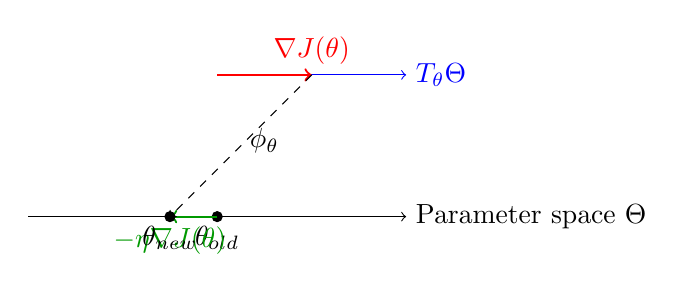
\begin{tikzpicture}[scale=1.2]
% Parameter space
\draw[->] (0,0) -- (4,0) node[right] {Parameter space $\Theta$};
\filldraw (2,0) circle (1.5pt) node[below] {$\theta_{\text{old}}$};

% Tangent space
\draw[->, blue] (2,1.5) -- (4,1.5) node[right] {$T_\theta\Theta$};
\draw[->, thick, red] (2,1.5) -- (3,1.5) node[above] {$\nabla J(\theta)$};

% Update
\draw[->, thick, green!60!black] (2,0) -- (1.5,0) node[below] {$-\eta\nabla J(\theta)$};
\filldraw (1.5,0) circle (1.5pt) node[below] {$\theta_{\text{new}}$};

% Isomorphism
\draw[dashed, ->] (3,1.5) -- (1.5,0);
\node at (2.5,0.8) {$\phi_\theta$};
\end{tikzpicture}
\caption{The gradient descent update implicitly uses the isomorphism between tangent space and parameter space.}
\end{figure}

\subsection{When the Standard Approach Fails}

The standard gradient descent assumes $\Theta = \mathbb{R}^n$. This fails when:

\subsubsection{Constrained Optimization}
If $\theta$ must satisfy $g(\theta) = 0$, then:
\begin{itemize}
\item Parameter space: $\{\theta \in \mathbb{R}^n : g(\theta) = 0\}$ (a manifold)
\item Gradient update may leave the constraint surface
\item Solution: Projected gradient descent or manifold optimization
\end{itemize}

\subsubsection{Natural Gradient}
\begin{itemize}
\item Uses Fisher information matrix $G(\theta)$ as Riemannian metric
\item Update: $\theta_{\text{new}} = \theta_{\text{old}} - \eta G(\theta)^{-1} \nabla J(\theta)$
\item Respects the information geometry of the parameter space
\end{itemize}

\subsubsection{Optimization on Manifolds}
Examples:
\begin{itemize}
\item Stiefel manifolds: $\{\theta \in \mathbb{R}^{n \times p} : \theta^\top\theta = I\}$
\item Sphere: $\{\theta \in \mathbb{R}^n : \|\theta\| = 1\}$
\item Requires Riemannian optimization techniques
\end{itemize}

\subsection{Practical Example: Optimization on a Sphere}

Let $\Theta = S^{n-1} = \{\theta \in \mathbb{R}^n : \|\theta\| = 1\}$.

\begin{itemize}
\item Parameter space: Sphere surface
\item Tangent space at $\theta$: $T_\theta S^{n-1} = \{v \in \mathbb{R}^n : \theta^\top v = 0\}$
\item Euclidean gradient $\nabla J(\theta)$ may point off the sphere
\item Must project to tangent space: $P_\theta(\nabla J(\theta)) = \nabla J(\theta) - (\theta^\top \nabla J(\theta))\theta$
\item Then update along geodesic or retract back to sphere
\end{itemize}

\subsection{The General Principle}

The correct geometric update is:
\[
\theta_{\text{new}} = R_\theta(-\eta \cdot \text{grad} J(\theta))
\]
where:
\begin{itemize}
\item $\text{grad} J(\theta)$ is the Riemannian gradient (in $T_\theta\Theta$)
\item $R_\theta: T_\theta\Theta \to \Theta$ is a retraction mapping tangent vectors to points
\end{itemize}

In Euclidean space, $R_\theta(v) = \theta + v$ is a natural retraction.
\end{notechapter}
